\documentclass{article}



\usepackage{fullpage}
%\usepackage{nopageno}
\usepackage{amsmath}
\usepackage{amsfonts}
\usepackage{graphicx}
\usepackage{framed}
\usepackage{xcolor}

\definecolor{dark_red}{rgb}{0.5,0.0,0.0}
\definecolor{dark_green}{rgb}{0.0,0.5,0.0}
\definecolor{dark_blue}{rgb}{0.0,0.0,0.5}
\definecolor{blue}{rgb}{0.0,0.0,1.0}

\newcommand{\cis}{\textnormal{cis}\,}
\newcommand{\dr}[1]{\textcolor{dark_red}{#1}}
\newcommand{\dg}[1]{\textcolor{dark_green}{#1}}
\newcommand{\db}[1]{\textcolor{dark_blue}{#1}}
\newcommand{\blue}[1]{\textcolor{blue}{#1}}


\begin{document}

\section*{Addition vs Multiplication}

Multiplication bears many similarities to addition:

\begin{itemize}
%%%%%%%%%%%%%%%%%%%%%%%%%%%
\item Addition and multiplication are both commutative.
\[\forall a, b \in \mathbb{R} : (a + b = b + a) \;\wedge\; (a \cdot b = b \cdot a)\]
\begin{center}\textbf{``for all choices of real numbers \(a\) and \(b\), it is the case that \(a + b = b + a\) and \(a \cdot b = b \cdot a\)"}\end{center}
%%%%%%%%%%%%%%%%%%%%%%%%%%%
\item Addition and multiplication are both associative.
\[\forall a, b, c \in \mathbb{R} : ((a + b) + c = a + (b + c)) \;\wedge\; ((a \cdot b) \cdot c = a \cdot (b \cdot c))\]
\begin{center}\textbf{``for all choices of real numbers \(a\), \(b\), and \(c\), it is the case that \((a + b) + c = a + (b + c)\) and \((a \cdot b) \cdot c = a \cdot (b \cdot c)\)"}\end{center}
%%%%%%%%%%%%%%%%%%%%%%%%%%%
\item Adding \(0\) to a number does not change the number, and multiplying \(1\) onto a number does not change the number. \(1\) is the multiplication equivalent of \(0\).
\[\forall a \in \mathbb{R} : (a + 0 = a) \;\wedge\; (a \cdot 1 = a)\]
\begin{center}\textbf{``for all choices of real number \(a\), it is the case that \(a + 0 = a\) and \(a \cdot 1 = a\)"}\end{center}
%%%%%%%%%%%%%%%%%%%%%%%%%%%
\item Every real number as a negative, and every nonzero number has a reciprocal. The negative of a number when added to the original number results in \(0\):
\[\forall a \in \mathbb{R} : (a + (-a) = 0)\]
\begin{center}\textbf{``for all choices of real number \(a\), it is the case that \(a + (-a) = 0\)"}\end{center}
The reciprocal of a nonzero number when multiplied by the original number results in \(1\):
\[\forall a \in \mathbb{R} : a \neq 0 \implies (a \cdot \frac{1}{a} = 1)\]
\begin{center}\textbf{``for all choices of real number \(a\), if \(a \neq 0\) then \(a \cdot \frac{1}{a} = 1\)"}\end{center}
%%%%%%%%%%%%%%%%%%%%%%%%%%%
\item Moreover, subtraction is the addition of a negative:
\[\forall a, b \in \mathbb{R} :  a - b = a + (-b)\] 
\begin{center}\textbf{``for all choices of real numbers \(a\) and \(b\), it is the case that \(a - b = a + (-b)\)"}\end{center} 
and division is the multiplication of a reciprocal:
\[\forall a, b \in \mathbb{R} :  b \neq 0 \implies (a / b = a \cdot \frac{1}{b})\] 
\begin{center}\textbf{``for all choices of real numbers \(a\) and \(b\), if \(b \neq 0\) then \(a / b = a \cdot \frac{1}{b}\)"}\end{center} 
\end{itemize}



\section*{The difficulties of multiplication}

Despite multiplication and addition being similar in many respects, multiplication is a much more complicated operation to perform by hand than is addition. Before the widespread use of calculators, multiplying together to numbers directly is prohibitively difficult.

%Consider for example the two 8-digit numbers \(a = 74307261\) and \(b = 11567239\).
%
%The addition of the two numbers simply involves adding the digits from least significant to most significant, propagating carries if necessary. The {\bf number of steps} is proportional to the {\bf sum} of the lengths (number of digits) of \(a\) and \(b\).
%
%\begin{align*}
%\begin{array}{ccccccccc}
%    & 7 & 4 & 3 & 0 & 7 & 2 & 6 & 1 \\ 
%+ & 1 & 1 & 5 & 6 & 7 & 2 & 3 & 9 \\ 
%\hline
%0 & 8 & 5 & 8 & 7 & 4 & 5 & 0 & 0
%\end{array}
%\end{align*}
%
%In contrast, the multiplication of the two numbers involves the computing of partial products for each pair of digits, and the summation of the results. The {\bf number of steps} is proportional to the {\bf product} of the lengths (number of digits) of \(a\) and \(b\). This becomes prohibitively large as \(a\) and \(b\) increase in length.
%
%%0 x 74307261 = 000000000
%%1 x 74307261 = 074307261
%%                           074307261
%%2 x 74307261 = 148614522
%%                           074307261
%%3 x 74307261 = 222921783
%%                           074307261
%%4 x 74307261 = 297229044
%%                           074307261
%%5 x 74307261 = 371536305
%%                           074307261
%%6 x 74307261 = 445843566
%%                           074307261
%%7 x 74307261 = 520150827
%%                           074307261
%%8 x 74307261 = 594458088
%%                           074307261
%%9 x 74307261 = 668765349
%
%\begin{align*}
%\begin{array}{cccccccccccccccc}
%& & & & & & &            & 7 & 4 & 3 & 0 & 7 & 2 & 6 & 1 \\ 
%& & & & & & & \times & 1 & 1 & 5 & 6 & 7 & 2 & 3 & 9 \\ 
%\hline
%& & & & & &    & 6 & 6 & 8 & 7 & 6 & 5 & 3 & 4 & 9
%                    2 & 2 & 2 & 9 & 2 & 1 & 7 & 8 & 3 & 0
%              1 & 4 & 8 & 6 & 1 & 4 & 5 & 2 & 2 & 0 & 0
%\end{array}
%\end{align*}

Consider for example the two 4-digit numbers \(a = 7430\) and \(b = 1956\).

The addition of the two numbers simply involves adding the digits from least significant to most significant, propagating carries if necessary. The {\bf number of steps} is proportional to the {\bf sum} of the lengths (number of digits) of \(a\) and \(b\).

\begin{align*}
\begin{array}{ccccc}
    & 7 & 4 & 3 & 0 \\ 
+ & 1 & 9 & 5 & 6 \\ 
\hline
0 & 9 & 3 & 8 & 6
\end{array}
\end{align*}

In contrast, the multiplication of the two numbers involves the computing of partial products for each pair of digits, and the summation of the results. The {\bf number of steps} is proportional to the {\bf product} of the lengths (number of digits) of \(a\) and \(b\). This becomes prohibitively large as \(a\) and \(b\) increase in length.

%0 x 7430 = 00000
%1 x 7430 = 07430
%                     7430
%2 x 7430 = 14860
%                     7430
%3 x 7430 = 22290
%                     7430
%4 x 7430 = 29720
%                     7430
%5 x 7430 = 37150
%                     7430
%6 x 7430 = 44580
%                     7430
%7 x 7430 = 52010
%                     7430
%8 x 7430 = 59440
%                     7430
%9 x 7430 = 66870

\begin{align*}
\begin{array}{cccccccc}
& & &            & 7 & 4 & 3 & 0 \\ 
& & & \times & 1 & 9 & 5 & 6 \\ 
\hline
   &    &    & 4 & 4 & 5 & 8 & 0 \\
   &    & 3 & 7 & 1 & 5 & 0 & 0 \\
   & 6 & 6 & 8 & 7 & 0 & 0 & 0 \\
0 & 7 & 4 & 3 & 0 & 0 & 0 & 0 \\
\hline
1 & 4 & 5 & 3 & 3 & 0 & 8 & 0 
\end{array}
\end{align*}



\section*{The logarithm}

To address the challenges of multiplication, the similarities of multiplication to addition can be used to assign to each number a ``multiplicative essence". {\bf The term ``multiplicative essence" is used only in this document, and is not recognized officially.} The multiplicative essence can be extracted through use of the {\bf logarithm}. Given an arbitrary {\bf positive} number \(x\), \(\log(x)\) is the ``multiplicative essence" of \(x\). When multiplying two positive real numbers \(x\) and \(y\), the multiplicative essence of the product is the {\bf sum} of the multiplicative essences of the factors, the sum of two numbers being much easier to compute. {\bf Using logarithms turns multiplication into addition}:

\begin{itemize}
\item Multiplying two numbers can be performed by adding their logarithms. For any choice of positive numbers \(x\) and \(y\), 
\[\log(x \cdot y) = \log(x) + \log(y)\]
\item \(1\) is the multiplication analog to \(0\), so
\[\log(1) = 0\]
\item The reciprocal is the multiplication analog to the negative, so for any positive number \(x\), 
\[\log(1/x) = -\log(x)\]
\item Division is the multiplication analog to subtraction. For any choice of positive numbers \(x\) and \(y\), 
\[\log(x / y) = \log(x) - \log(y)\]
\item Multiplying a number \(x\) by itself \(n\) times is defined as \(x^n\). The logarithm of \(x^n\) is the logarithm of \(x\) {\bf added} to itself \(n\) times. For any positive number \(x\), and natural number \(n\),
\[\log(x^n) = \log(\underbrace{x \cdot x \cdot ... \cdot x}_n) = \underbrace{\log(x) + \log(x) + ... + \log(x)}_n = n \cdot \log(x)\]
If \(r\) is an arbitrary real number, then 
\[\log(x^r) = r \cdot \log(x)\]
also.
\item The \(n^\text{th}\) root of a positive number \(x\), denoted by \(\sqrt[n]{x}\), is a number that when multiplied by itself \(n\) times yields \(x\). The logarithm of \(\sqrt[n]{x}\) when added to itself \(n\) times yields the logarithm of \(x\), so \(n \cdot \log(\sqrt[n]{x}) = \log(x)\) which then yields:
\[\log(\sqrt[n]{x}) = \frac{1}{n}\log(x)\]
\end{itemize}

Even with the above properties, the logarithm is not yet fully defined. The choice that remains is to choose a ``base" for the logarithm. The base \(b\) is the number whose multiplicative essence is \(1\) (the multiplicative essence of 1 is 0): \(\log(b) = 1\). The base \(b\) should always be a positive real number greater than \(1\). The notation \(\log_b(x)\) is the logarithm of \(x\) using base \(b\). \(\log_b(x)\) is the multiplicative essence of \(x\) where the multiplicative essence of \(b\) is calibrated to \(1\). It goes by definition that \(\log_b(b) = 1\). Moreover for any real number \(r\) the multiplicative essence of \(b^r\) is \(r\): 
\[\log_b(b^r) = r \cdot \log_b(b) = r \cdot 1 = r\]
Given an arbitrary multiplicative essence \(r\), the number that has a multiplicative essence of \(r\) is \(b^r\). \(b^r\) is sometimes referred to as the {\bf antilogarithm} of \(r\). If function \(f(X)\) is defined as \(f(X) = \log_b(X)\), then the inverse of \(f\) is \(f^{-1}(Y) = b^Y\).

The graph on the right illustrates how the base \(b\) logarithm of \(x\) changes with \(x\). The logarithm only exists for positive values of \(x\). The logarithm increases with \(x\), and every real number is in the range of possible logarithms. 

\begin{tabular}{cc}
\parbox{0.5\textwidth}{
\begin{itemize}
\item When \(x = 1\), \(\log_b(1) = 0\), since \(1\) is the multiplication analog to \(0\).
\item When \(x\) decreases from \(1\) to \(0\), \(\log_b(x)\) decreases from \(0\) to \(-\infty\). When \(0 < x < 1\), multiplying a number by \(x\) decreases the magnitude of said number, so a negative logarithm makes sense. 
\item When \(x\) increases from \(1\) to \(b\), \(\log_b(x)\) increases from \(0\) to \(1\). When \(1 < x < b\), multiplying a number by \(x\) increases its magnitude, but not as much as a multiplication by \(b\) or higher. Hence a positive logarithm that is less than \(1\) makes sense. 
\end{itemize}
} & \parbox{0.5\textwidth}{
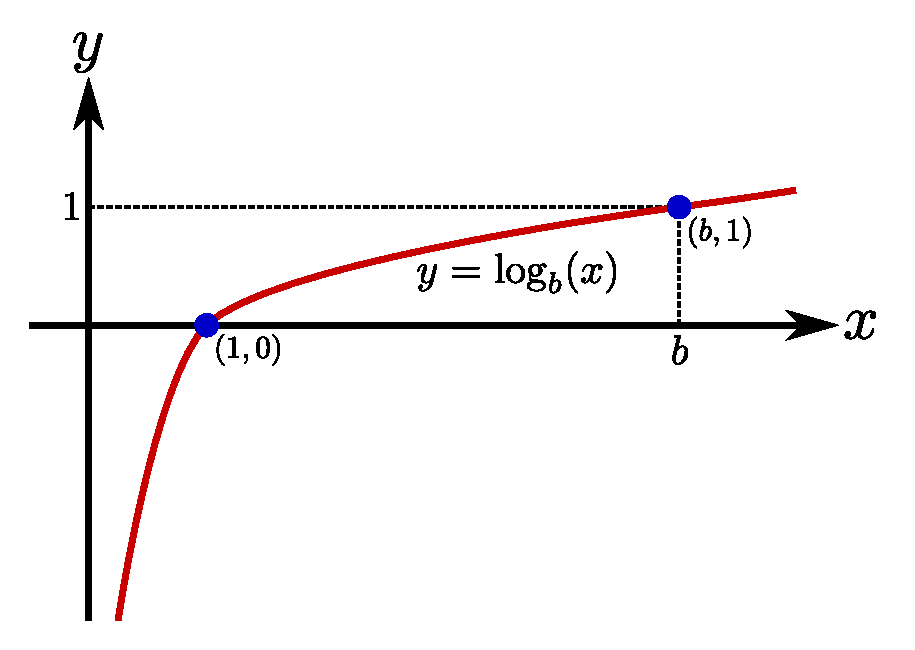
\includegraphics[width = 0.5\textwidth]{logarithm_graph}
}
\end{tabular}
\begin{itemize}
\item When \(x = b\), \(\log_b(b) = 1\) by definition of the base.
\item When \(x\) increases past \(b\), \(\log_b(x)\) increases past \(1\) and very slowly increases to \(+\infty\). When \(x > b\), multiplying a number by \(x\) increases its magnitude more than a multiplication by \(b\), so a logarithm greater than \(1\) makes sense.
\end{itemize}

Common bases include \(10\), \(2\), and ``\(e\)". The number ``\(e\)" is Euler's constant and will be covered later.

Base \(2\) is often used when measuring information as a number of ``bits" (binary digits).

Base \(10\) is what was used to quicken the process of multiplication before the use of calculators, as will be covered below. 

Base \(e\) has a very important property that is invaluable to algebra and Calculus, and will be covered later.

To help further illustrate logarithm values, the base \(10\) logarithms for several numbers are shown below:

\begin{tabular}{|c||c|c|c|c|c|}
\hline
\(x\) & 0.1 & 0.2 & 0.3 & 0.4 & 0.5 \\
\hline
\(\log_{10}(x)\) & -1 & -0.698970 & -0.522879 & -0.397940 & -0.301030 \\
\hline
\hline
\(x\) & 0.6 & 0.7 & 0.8 & 0.9 & 1.0 \\
\hline
\(\log_{10}(x)\) & -0.221849 & -0.154902 & -0.0969100 & -0.0457575 & 0 \\
\hline
\hline
\(x\) & 2.0 & 3.0 & 4.0 & 5.0 & 6.0 \\
\hline
\(\log_{10}(x)\) & 0.301030 & 0.477121 & 0.602060 & 0.698970 & 0.778151 \\
\hline
\hline
\(x\) & 7.0 & 8.0 & 9.0 & 10.0 & 20.0 \\
\hline
\(\log_{10}(x)\) & 0.845098 & 0.903090 & 0.954243 & 1 & 1.30103 \\
\hline
\end{tabular}

\vspace{5mm}

What if a change of base is needed? If we have the logarithm of \(x\) in base \(b\), i.e. \(\log_b(x)\), and we need the logarithm of \(x\) in base \(c\), i.e. \(\log_c(x)\), then just like converting between units, the following is performed. Given the base \(b\) logarithm \(\log_b(x)\) and some arbitrary constant \(k\), then the expression \(\log_?(x) = k \cdot \log_b(x)\) also computes a valid logarithm, albeit one where the logarithm when \(x = b\) is no longer calibrated to \(1\). The expression \(\frac{1}{\log_b(c)} \log_b(x)\) is a valid logarithm that evaluates to \(1\) when \(x = c\). The expression \(\frac{1}{\log_b(c)} \log_b(x)\) is a logarithm where the logarithm of \(c\) is calibrated to \(1\). Therefore:
\[\log_c(x) = \frac{\log_b(x)}{\log_b(c)}\]   
In other words, \(\log_c(x)\) is the logarithm of \(x\), i.e. \(\log_b(x)\), measured in units of the logarithm of \(c\), i.e. \(\log_b(c)\).





\section*{Before there were calculators...}

\subsection*{Log tables}

As noted in the previous sections, multiplying numbers by hand before the use of calculators was prohibitively difficult. Fortunately, if one is willing to allow some approximations, logarithms can be used to convert the difficult task of multiplication into the much simpler task of addition. Base \(10\) logarithms are used. Base \(10\) logarithms are referred to as ``common logarithms" and are the default for the ``\texttt{log}" key found on most calculators. Why are base \(10\) logarithms used to simplify multiplication and not some other base? The answer is that finding the base \(10\) logarithm of a number in {\bf scientific notation} is easy when paired with a ``log table".

\begin{tabular}{cc}
\parbox{0.5\textwidth}{
A ``log table" is a lengthy book that lists the logarithms for a vast range of numbers. A fragment of a such a log table is displayed on the right. For the purpose of this discussion, we will assume that the log table will allow the quick determination of the logarithm \(\log_{10}(x)\) of numbers from the range \([1, 10)\), and the quick determination of the antilogarithm \(10^x\) of numbers from the range \([0, 1)\). 
} & \parbox{0.5\textwidth}{
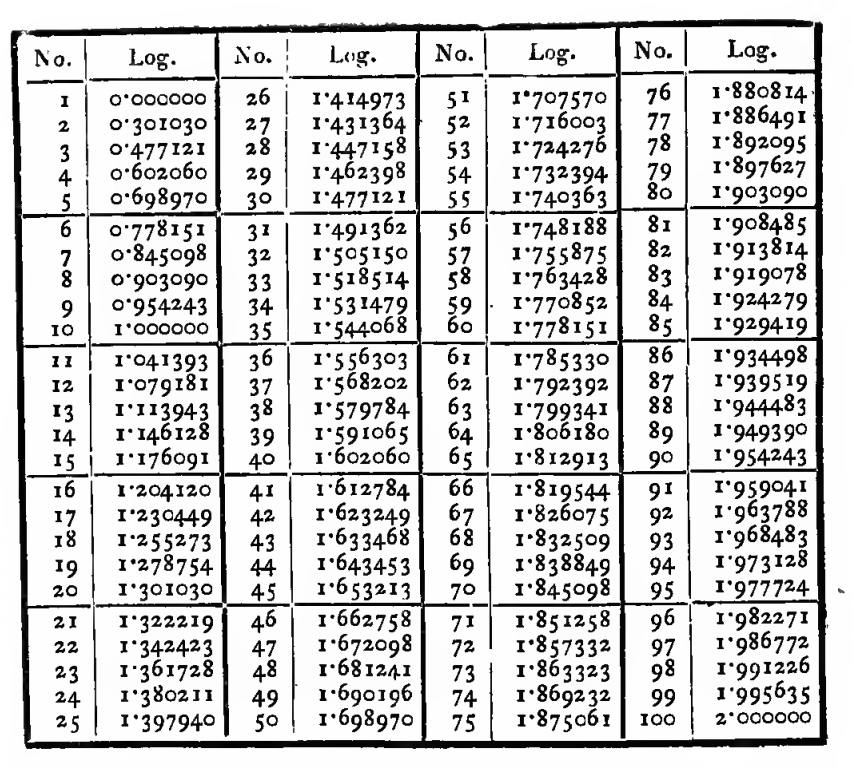
\includegraphics[width = 0.5\textwidth]{Log_table_fragment.png}
} \\
& \parbox{0.5\textwidth}{\footnotesize Image credit: Wikimedia Commons, URL: 
{\textless
https://commons.wikimedia.org/wiki/File:Tables\_of\_six-figure\_logarithms\_(IA\_cu31924031296795).pdf
\textgreater}
}
\end{tabular} 
\begin{itemize}
%%%%%%%%%%%%%%%%%
\item To use the log table to compute the logarithm of an arbitrary positive number \(x\), the number will be expressed in scientific notation: 
\[x = +a \times 10^n\] where the exponent \(n\) is an integer and the coefficient \(a \in [1, 10)\) is the ``{\bf mantissa}". 
The base \(10\) logarithm of \(x\) is 
\begin{align*}
\log_{10}(x) = \log_{10}(+a \times 10^n) = \log_{10}(a) + \log_{10}(10^n) = n + \log_{10}(a)
\end{align*} 
where \(\log_{10}(a)\) is computed from the log table. \(\log_{10}(a)\) belongs to the interval \([0, 1)\), and is the fractional part of the logarithm. 
%%%%%%%%%%%%%%%%%
\item To use the log table to compute the antilogarithm of an arbitrary number \(y\), the number will be expressed in the form: 
\[y = n + r\] where \(n\) is an integer and \(r \in [0, 1)\). 
The base \(10\) antilogarithm is 
\[10^y = 10^{n+r} = +10^r \times 10^n\]
where \(10^r\) is computed from the log table. \(10^r\) belongs to the interval \([1, 10)\), and becomes the mantissa.
\end{itemize}
This is how log tables allow the quick calculations of base 10 logarithms and antilogarithms. 

\vspace{5mm}

\begin{description}
\item[Example 1:] ~

Consider the process of multiplying the numbers \(x = 5.67128 \times 10^8\) and \(y = 1.04690 \times 10^3\). 

The logarithm (multiplication essence) of \(x\) is: 
\[\log_{10}(x) = \log_{10}(5.67128 \times 10^8) = 8 + \log_{10}(5.67128) \approx 8 + 0.753681 = 8.753681\]
The logarithm (multiplication essence) of \(y\) is:
\[\log_{10}(y) = \log_{10}(1.04690 \times 10^3) = 3 + \log_{10}(1.04690) \approx 3 + 0.019905 = 3.019905\]
With the logarithms of \(x\) and \(y\) now known (to an approximation), the logarithm of the product \(xy\) is the sum of the logarithms:
\[\log_{10}(xy) = \log_{10}(x) + \log_{10}(y) \approx 8.753681 + 3.019905 = 11.773586\]
Now is time to compute the ``antilogarithm" and extract the final product \(xy\). The logarithm of the product is, 
\[11.773586 = 11 + 0.773586\]
so
\[xy \approx 10^{11 + 0.773586} = 10^{0.773586} \times 10^{11} \approx 5.93726 \times 10^{11}\]
Therefore
\[(5.67128 \times 10^8)(1.04690 \times 10^3) \approx 5.93726 \times 10^{11}\]


\item[Example 2:] ~

As another example, let \(x = 2.45207 \times 10^2\) and \(y = 6.89641 \times 10^4\), and then compute the quotient \(x/y\). 

The logarithm (multiplication essence) of \(x\) is: 
\[\log_{10}(x) = \log_{10}(2.45207 \times 10^2) = 2 + \log_{10}(2.45207) \approx 2 + 0.389533 = 2.389533\]
The logarithm (multiplication essence) of \(y\) is: 
\[\log_{10}(y) = \log_{10}(6.89641 \times 10^4) = 4 + \log_{10}(6.89641) \approx 4 + 0.838623 = 4.838623\]
With the logarithms of \(x\) and \(y\) now known (to an approximation), the logarithm of the quotient \(x/y\) is the difference of the logarithms:
\[\log_{10}(x/y) = \log_{10}(x) - \log_{10}(y) \approx 2.389533 - 4.838623 = -2.449090\]
Now is time to compute the ``antilogarithm" and extract the final quotient \(x/y\). The logarithm of the product is, 
\[-2.449090 = -3 + 0.550910\]
so
\[\frac{x}{y} \approx 10^{-3 + 0.550910} = 10^{0.550910} \times 10^{-3} \approx 3.55558 \times 10^{-3}\]
Therefore
\[\frac{2.45207 \times 10^2}{6.89641 \times 10^4} \approx 3.55558 \times 10^{-3}\]


\item[Example 3:] ~

As a last example, let \(x = 2.68194 \times 10^7\) and \(y = -4.57891\), and then compute \(x^y\). 

The logarithm (multiplication essence) of \(x\) is: 
\[\log_{10}(x) = \log_{10}(2.68194 \times 10^7) = 7 + \log_{10}(2.68194) \approx 7 + 0.428449 = 7.428449\]

\(\log_{10}(x)\) is now to be multiplied by \(y\). Once again there is a tough multiplication problem. The logarithm of \(\log_{10}(x)\) is:
\[\log_{10}(\log_{10}(x)) \approx \log_{10}(7.428449) \approx 0.870898\]
\(y\) is negative, so the logarithm of \(|y|\) is computed instead. The sign will be reincorporated later. 
\[\log_{10}(|y|) = \log_{10}(4.57891) \approx 0.660762\]
The logarithm of the product \(|y|\log_{10}(x)\) is:
\begin{align*}
\log_{10}(|y|\log_{10}(x)) = & \log_{10}(|y|) + \log_{10}(\log_{10}(x)) \approx 0.660762 + 0.870898 = 1.531660 \\
= & 1 + 0.531660
\end{align*}
Computing the antilogarithm gives the product:
\[|y|\log_{10}(x) \approx 10^{1 + 0.531660} = 10^{0.531660} \times 10^1 \approx 3.401418 \times 10^1\]
so the logarithm of \(x^y\) is:
\[y\log_{10}(x) \approx -3.401418 \times 10^1 = -34.01418 = -35 + 0.98582\]
therefore:
\[x^y \approx 10^{-35 + 0.98582} = 10^{0.98582} \times 10^{-35} \approx 9.67877 \times 10^{-35}\]
\[(2.68194 \times 10^7)^{-4.57891} \approx 9.67877 \times 10^{-35}\]

\end{description}



\subsection*{Slide rules}

As an alternative to using log tables to perform multiplication, there is the analog tool known as the ``slide rule". The slide rule consists of a pair of marked straight edges where length corresponds to the logarithms, and the markings correspond to the original numbers (the antilogarithm). One such slide is depicted below:

\begin{center}
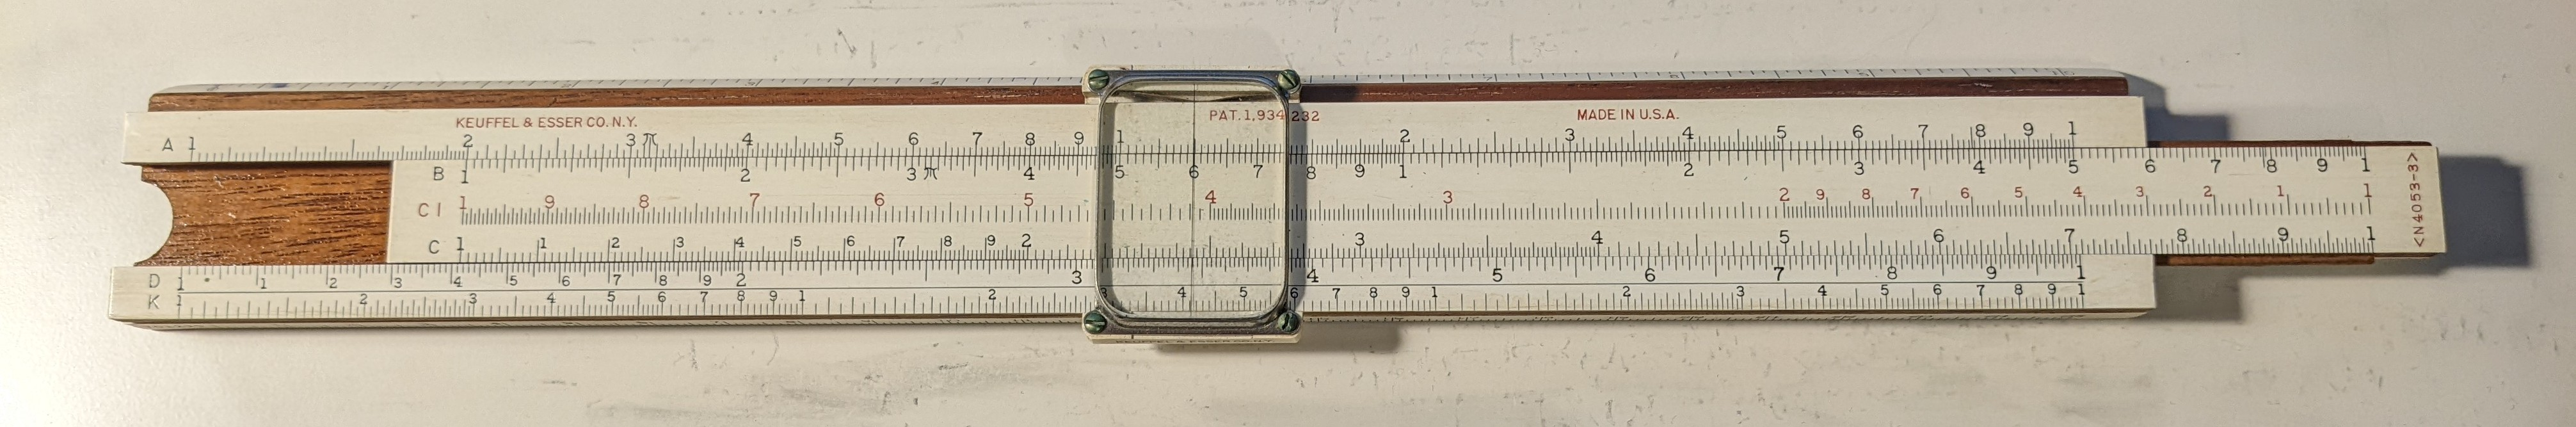
\includegraphics[width = \textwidth]{slide_rule_picture.jpg}
\end{center}    

In its default state, the slide rule scales are aligned as depicted below. Many slide rules have scales that run from \(1\) to \(100\), so any pair of mantissas from the range \([1, 10)\) can be multiplied. The numbers \(x\) and \(y\) are marked to be used in examples.

\begin{center}
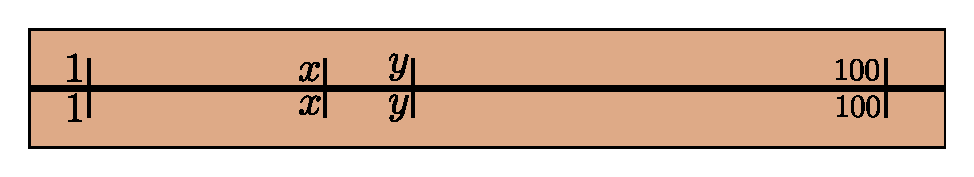
\includegraphics[scale = 0.5]{slide_rule}
\end{center}    

When two numbers \(x\) and \(y\) are to be multiplied, the lower scale is slid to the right until the \(1\) marking on the lower scale aligns with the \(x\) marking on the upper scale. The number on the upper scale that aligns with the \(y\) marking on the lower scale is the product \(xy\). 

\begin{center}
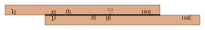
\includegraphics[scale = 0.5]{slide_rule_multiplication}
\end{center}   

When the quotient \(y/x\) is to be computed, the lower scale is slid to the right until the \(x\) marking on the lower scale aligns with the \(y\) marking on the upper scale. The number on the upper scale that aligns with the \(1\) marking on the lower scale is the quotient \(y/x\). 

\begin{center}
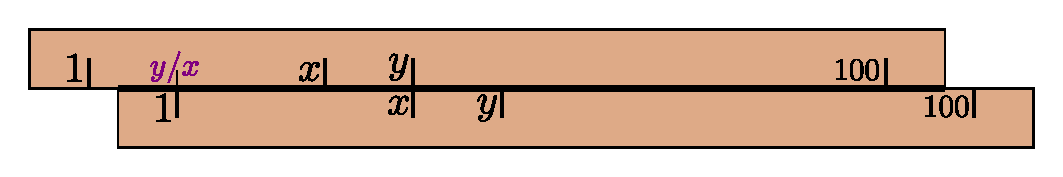
\includegraphics[scale = 0.5]{slide_rule_division}
\end{center}   

When the reciprocal \(1/x\) is to be computed, the lower scale is slid to the right until the \(x\) marking on the lower scale aligns with the \(100\) marking on the upper scale. The number on the upper scale that aligns with the \(1\) marking on the lower scale is the quotient \(100/x\). Shifting the decimal point 2 positions to the left yields the reciprocal \(1/x\). 

\begin{center}
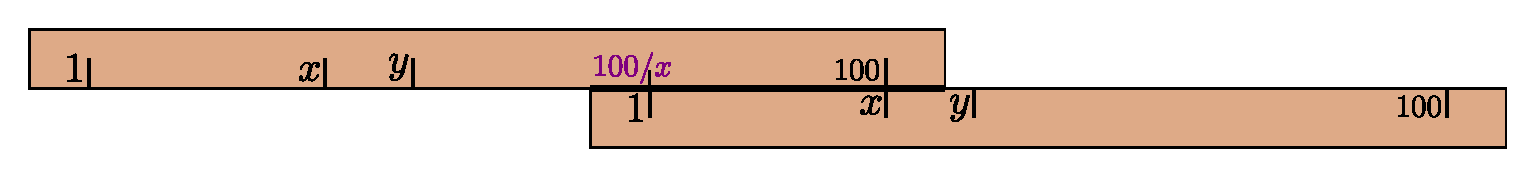
\includegraphics[scale = 0.5]{slide_rule_reciprocal}
\end{center} 





\section*{Natural logarithms}

The natural logarithm, which is denoted by the symbol \(\ln\) instead of \(\log\), is a logarithm where the following approximation holds:

For a number \(\epsilon\) that is very close to \(0\), the {\bf relative error} in the approximation 
\[\ln(1 + \epsilon) \approx \epsilon\]
is very close to \(0\).

As a reminder, the relative error is an error measure where the magnitude of the difference is divided by either the approximation or true value to get a number which measures the fraction (commonly expressed as a percentage) of the approximation that is actually error, or by what fraction of the true value the approximation misses its mark.

\[\textbf{relative\_error} = \frac{|\textbf{approximation} - \textbf{true\_value}|}{|\textbf{approximation}|} \quad\text{or}\quad \textbf{relative\_error} = \frac{|\textbf{approximation} - \textbf{true\_value}|}{|\textbf{true\_value}|}\]

Why is the approximation \(\ln(1 + \epsilon) \approx \epsilon\) important? This approximation enables the approximation of the logarithm for values that are close to \(1\), \(1\) being the multiplication equivalent of \(0\). 

The base that the natural logarithm uses is denoted by ``\(e\)", referred to as ``Euler's constant". To home-in on the actual value of \(e\), let \(N\) denote a very large positive number. \(\frac{1}{N}\) is close to \(0\), so 
\[\ln\left(1 + \frac{1}{N}\right) \approx \frac{1}{N} \implies N \cdot \ln\left(1 + \frac{1}{N}\right) \approx N \cdot \frac{1}{N} \implies \ln\left(\left(1 + \frac{1}{N}\right)^N\right) \approx 1\]
The base \(e\) of the natural logarithm is approximately \(\left(1 + \frac{1}{N}\right)^N\), the approximation becoming more accurate as \(N\) increases. The table below shows the value of \(\left(1 + \frac{1}{N}\right)^N\) converging on \(e\) as \(N\) increases:
\begin{tabular}{|c||c|c|c|c|c|c|c|c||c|}
\hline
\(N\)                                               & \(1\) & \(2\)      & \(3\)            & \(4\)             & \(5\)            & \(6\)            & \(7\)             & \(20\)          & \(+\infty\) \\
\hline
\(\left(1 + \frac{1}{N}\right)^N\) & \(2\) & \(2.25\) & \(2.37037\) & \(2.44141\) & \(2.48832\) & \(2.52163\) & \(2.54650\) & \(2.65330\) & \(e = 2.71828...\) \\
\hline
\end{tabular}

\vspace{5mm}

Given a series of small numbers \(\epsilon_1, \epsilon_2, ..., \epsilon_N\), the product 
\[P = (1 + \epsilon_1)(1 + \epsilon_2)...(1 + \epsilon_N)\]
can be simplified through the use of the natural logarithm. For each \(i = 1, 2, ..., N\), the natural logarithm of the \(i^\text{th}\) factor is \(\ln(1 + \epsilon_i) \approx \epsilon_i\). The logarithm of the entire product is:
\begin{align*}
\ln(P) = & \ln((1 + \epsilon_1)(1 + \epsilon_2)...(1 + \epsilon_N)) 
= \ln(1 + \epsilon_1) + \ln(1 + \epsilon_2) + \cdots + \ln(1 + \epsilon_N) \\
\approx & \epsilon_1 + \epsilon_2 + \cdots + \epsilon_N
\end{align*}
Therefore the product is:
\[(1 + \epsilon_1)(1 + \epsilon_2)...(1 + \epsilon_N) = P \approx e^{\epsilon_1 + \epsilon_2 + \cdots + \epsilon_N}\]  

\vspace{5mm}



\textbf{Example applications:}

\begin{description}
\item[The lottery:] ~ 

If the lottery odds are \(1\) in \(N\) where \(N\) is a large number such as \(N = 10000000\), it is commonly assumed that buying \(N\) tickets will guarantee you a win. While the average number of wins from \(N\) tickets is indeed \(1\), at least \(1\) win is not guaranteed, contrary to naive expectations. What is the actual probability of winning from \(N\) tickets?

After buying \(1\) ticket, the probability of losing is \(1 - \frac{1}{N}\). After buying \(N\) tickets, the probability of losing is cumulatively \(P = \left(1 - \frac{1}{N}\right)^N\) and this is nonzero. With the use of the natural logarithm, \(P\) can be approximated. Each factor \(1 - \frac{1}{N}\) is close to \(1\), so the natural logarithm can be used to multiply these factors. By definition of the natural logarithm, 
\[\ln\left(1 - \frac{1}{N}\right) \approx -\frac{1}{N}\]
so 
\[\ln(P) = \ln\left(\left(1 - \frac{1}{N}\right)^N\right) = N\ln\left(1 - \frac{1}{N}\right) \approx N \cdot \frac{-1}{N} = -1\]
With the natural logarithm of the probability of losing after \(N\) tickets being \(-1\), the probability of losing after \(N\) tickets is: 
\[e^{-1} = \frac{1}{e} \approx 36.7879\%\]
You only have a \(63.2121\%\) chance of winning after \(N\) tickets. 

Buying \(N\) tickets costs more than the payout, and you are still not guaranteed a win. Don't play the lottery. 



\item[Poisson processes:] ~
 
Consider a machine that is known to fail periodically. After careful experimentation, it is determined that the ratio of the number of failures to the length of time is on average, \(\lambda\) failures per unit of time. \(\lambda\) is referred to as the failure rate. Given an arbitrary time \(t\), the product \(\lambda t\) is the average number of failures that will occur within a time interval of length \(t\). It should be noted that \(\lambda t\) is the {\bf average} number of failures amongst all time intervals of length \(t\), and that the actual number of failures {\bf may vary}. What however, is the probability of avoiding a failure over a time interval of \(t\)? 

Let \(N\) be a very large natural number and divide the time interval of \(t\) into \(N\) tiny fragments of \(\Delta t = \frac{t}{N}\). The average number of failures in the tiny time interval \(\Delta t\) is \(\lambda\Delta t\). Since \(\Delta t\) is tiny and close to \(0\), the probability of scenarios of \(2\) or more failures in the time interval of \(\Delta t\) is negligible when compared to the probability of a single failure. The average number of failures \(\lambda\Delta t\) becomes the probability of {\bf any} failure occurring in the time interval \(\Delta t\). 

The probability of no failure in a time interval of \(\Delta t\) is \(1 - \lambda\Delta t\). The probability of no failure over \(N\) consecutive intervals of \(\Delta t\) culminates to \((1 - \lambda\Delta t)^N\). \(N\) consecutive intervals of \(\Delta t\) is the desired time interval \(t\). The probability of no failure over a time interval of \(t\) is 
\[P = (1 - \lambda\Delta t)^N\]  
This is the product of \(N\) quantities that are close to \(1\). To multiply these quantities that are close to \(1\), the natural logarithm of each factor of \(1 - \lambda\Delta t\) will be computed and then summed. Since \(-\lambda\Delta t\) is close to \(0\),
\[\ln(1 - \lambda\Delta t) \approx -\lambda \Delta t\]
The natural logarithm of the product is:
\[\ln(P) = \ln((1 - \lambda\Delta t)^N) = N\ln(1 - \lambda\Delta t) \approx N(-\lambda \Delta t) = -\lambda \cdot N\Delta t = -\lambda \cdot t\]
With the natural logarithm of the probability of no failure being \(-\lambda \cdot t\), the probability of no failure over a time interval of \(t\) is:
\[P = e^{-\lambda \cdot t}\] 

As an example, if \(\lambda = 0.000001\) failures per second, then the average number of failures per year, which is \(t \approx 3.15576 \times 10^7\text{s}\), is:  
\[\lambda t = 0.000001 \times (3.15576 \times 10^7) = 31.5576\]  
The probability of there being no failure for an entire year is: 
\[P = e^{-\lambda t} = e^{-31.5576} \approx 1.97110 \times 10^{-14}\]
With such low odds, a failure is basically certain. 


%\item[Air pressure:] ~
\end{description}




\section*{Logarithms and complex numbers}

The concept of logarithms will now be extended to complex numbers. A basic familiarity with complex numbers and polar coordinates will be assumed.

\subsection*{Review of complex numbers}

As a review, complex numbers consist of the sum of 2 components: a real component, and an imaginary component: 
\[z = x + i \cdot y\]
Visualizing a complex number as a 2D point, the real component \(x\) is the x-coordinate, and the imaginary component \(y\) is the y-coordinate. 

\vspace{5mm}

\begin{center}
\begin{tabular}{cc}
\parbox{0.5\textwidth}{
The addition of two complex numbers is simply the sum of the components: 
\begin{align*} 
z_1 + z_2 
= & (x_1 + i \cdot y_1) + (x_2 + i \cdot y_2)  
= (x_1 + x_2) + i \cdot (y_1 + y_2)
\end{align*} 

Multiplying a complex number \(z = x + i \cdot y\) by a real number \(c\) is performed by adding \(c\) copies of \(z\), which results in \(c\) copies of \(x\) plus \(c\) copies of \(i \cdot y\):
\[c \cdot z = c \cdot (x + i \cdot y) = cx + i \cdot cy\]
} & \parbox{0.5\textwidth}{
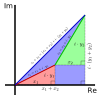
\includegraphics[scale = 0.7]{complex_number_addition}
}
\end{tabular}
\end{center}

The ``magnitude" \(|z|\) of a complex number \(z = x + i \cdot y\) is the distance of the point with Cartesian coordinates of \((x,y)\) from the origin: 
\[|z| = \sqrt{x^2 + y^2}\]

The multiplication of two complex numbers will be defined later.


\subsection*{Complex numbers and polar coordinates}

While complex numbers are often envisioned as the sum of a real and imaginary component, complex numbers can also be quantified using polar coordinates. A 2D point can be quantified using polar coordinates \(r\) and \(\theta\). 

\begin{center}
\begin{tabular}{cc}
\parbox{0.5\textwidth}{
The Cartesian coordinates associated with a point with polar coordinates \((r, \theta)\) is \((r\cos\theta, r\sin\theta)\). The complex number associated with this point is: 
\[z = r \cos\theta + i \cdot r\sin\theta = r(\cos\theta + i \cdot \sin\theta)\]
For simplicity, the expression \(\cos\theta + i \cdot \sin\theta\) is abbreviated using the notation \(\cis\theta\): 
\[\cis\theta = \cos\theta + i \cdot \sin\theta\]
so the complex number with polar coordinates \((r,\theta)\) is:
\[z = r \cdot \cis\theta\]
} & \parbox{0.5\textwidth}{
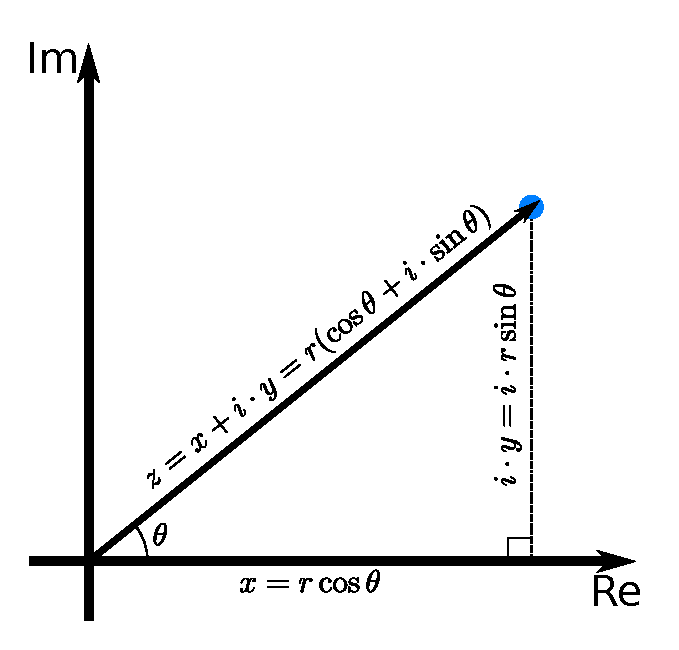
\includegraphics[scale = 0.7]{complex_number}
}
\end{tabular}
\end{center}


Now what about the multiplication of two complex numbers \(z_1 = x_1 + i \cdot y_1\) and \(z_2 = x_2 + i \cdot y_2\)? The polar representations of \(z_1\) and \(z_2\) will be assumed to be \(z_1 = r_1 \cis\theta_1\) and \(z_2 = r_2\cis\theta_2\).  

Using the distributive law, the product \(z_1 \cdot z_2\) is:
\begin{align*}
z_1 \cdot z_2 
= & z_1 (x_2 + i \cdot y_2) 
= z_1 x_2 + z_1 (i \cdot y_2)
\end{align*}
which is the sum of \(x_2\) copies of \(z_1\) followed by \(i \cdot y_2\) copies of \(z_1\). An \(i\) number of copies of \(z_1\) is a \(90^\circ\) counterclockwise rotation of \(z_1\). 

\(z_2\) is the sum of \(x_2\) copies of \(1\) and \(y_2\) copies of \(i\). 

Replacing each copy of \(1\) with \(z_1\) and each copy of \(i\) with \(i \cdot z_1\) has the effect of rotating \(z_2\) counter clockwise by \(\theta_1\) and increasing its length by a factor of \(r_1\), as depicted below. Therefore:
\begin{align*}
z_1 \cdot z_2 = & (r_1 r_2) \cis(\theta_1 + \theta_2)
\end{align*}

In summary, 
\[(r_1 \cis\theta_1)(r_2\cis\theta_2) = (r_1 r_2) \cis(\theta_1 + \theta_2)\]

\begin{center}
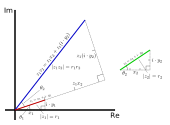
\includegraphics[width = 0.7\textwidth]{complex_number_multiplication}
\end{center}



\subsection*{Defining the logarithm of complex numbers}

It was previously observed that given \(z_1 = r_1 \cis\theta_1\) and \(z_2 = r_2\cis\theta_2\), then the product \(z_1 \cdot z_2\) is: 
\[z_1 \cdot z_2 = (r_1 \cis\theta_1)(r_2\cis\theta_2) = (r_1 r_2) \cis(\theta_1 + \theta_2)\]
To evaluate this product using only addition, the logarithms of \(r_1\) and \(r_2\) are to be added, and the angles \(\theta_1\) and \(\theta_2\) are to be simply added without any pre or post conversions. This gives the logarithm of a complex number \(z = r \cis\theta\) two pieces of information that have to be added separately: \(\log(r)\) and \(\theta\). The logarithm of \(z\) can be assigned a real component of \(\log(r)\) and an imaginary component of \(\theta\):

\[\log(r \cdot \cis\theta) = \log(r) + i \cdot k\theta\]
The coefficient \(k\) is determined by the unit of measurement for the angle \(\theta\). Angle \(\theta\) is measured in radians, but if degrees were the desired unit of measurement, then \(k = \frac{180^\circ}{\pi}\) to convert the radian measurement to degrees.

The focus will now be on defining the natural logarithm \(\ln(z)\). With regards to the natural logarithm \(\ln(z)\), the property \(\ln(1 + \epsilon) \approx \epsilon\) is still desired for values of the complex number \(\epsilon\) that are ``close" to \(0\). Right now the base \(b\) of the logarithm used for \(r\), and the unit of angle used for \(\theta\) is unknown, so
\[\ln(r \cdot \cis\theta) = \log_b(r) + i \cdot k\theta\]
where the base \(b\) and radians-to-unknown-angle-units conversion factor \(k\) still have be determined. 

Consider the complex number \(z = 1 + \epsilon = (1 + \epsilon_x) + i \cdot \epsilon_y\) where \(\epsilon = \epsilon_x + i \cdot \epsilon_y\) is close to \(0\). Approximations will be made that remain accurate even when the error is divided by, and therefore placed on the scale of, the length of \(\epsilon\), i.e. \(|\epsilon|\). 

Let \(r_\epsilon\) and \(\theta_\epsilon\) denote the polar coordinates of \(1 + \epsilon\), so \(1 + \epsilon = r_\epsilon\cis\theta_\epsilon\). 

In the image below, \(r_\epsilon\) is the radius of the red circular arc, and the approximation \(r_\epsilon \approx 1 + \epsilon_x\) can be observed. \(\theta_\epsilon\) is angle swept out by the red circular arc between the real line and \(1 + \epsilon\). The length of red circular arc swept out by \(\theta_\epsilon\) is \(r_\epsilon \cdot \theta_\epsilon\), using the formula for arc length, and this arc length is approximately \(\epsilon_y\) so the approximation \(r_\epsilon \cdot \theta_\epsilon \approx \epsilon_y\) can be observed.  

The approximation \(r_\epsilon \cdot \theta_\epsilon \approx \epsilon_y\) yields \(\theta_\epsilon \approx \frac{\epsilon_y}{r_\epsilon}\). Even though \(r_\epsilon\) is ``close" to \(1\), the approximation \(\frac{1}{r_\epsilon} \approx 1\) cannot be used since the error relative to \(|\epsilon|\) does not shrink to \(0\). However, the approximation \(\frac{\epsilon_y}{r_\epsilon} \approx \epsilon_y\) can still be used since multiplication by \(\epsilon_y\) makes the error vastly smaller.

Therefore:
\[r_\epsilon \approx 1 + \epsilon_x \quad\quad\text{and}\quad\quad \theta_\epsilon \approx \epsilon_y\]

\begin{center}
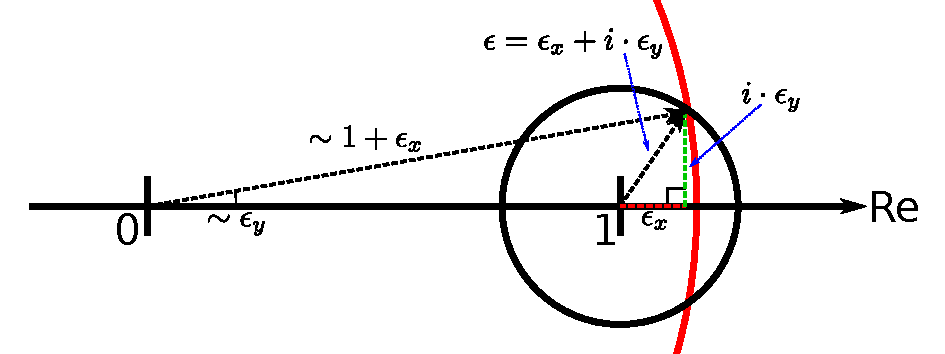
\includegraphics[width = 0.7\textwidth]{complex_number_natural_logarithm}
\end{center}

The condition:

\[\ln(1 + \epsilon) \approx \epsilon\] 

becomes

\[\ln(r_\epsilon \cis\theta_\epsilon) \approx \epsilon\] 

which becomes

\[\log_b(r_\epsilon) + i \cdot k\theta_\epsilon \approx \epsilon_x + i \cdot \epsilon_y\]

Using the approximations \(r_\epsilon \approx 1 + \epsilon_x\) and \(\theta_\epsilon \approx \epsilon_y\) gives:

\[\log_b(1 + \epsilon_x) + i \cdot k\epsilon_y \approx \epsilon_x + i \cdot \epsilon_y\]

For the real components to match, \(\log_b(1 + \epsilon_x) \approx \epsilon_x\), which necessitates the base \(b\) to be \(e\). 

For the imaginary components to match, \(k = 1\) so the angle in the logarithm is measured in radians. 

Therefore:
\[\ln(r \cis\theta) = \ln(r) + i \cdot \theta\]
and the property
\[\ln(1 + \epsilon) \approx \epsilon \quad\quad\textnormal{when \(\epsilon\) is close to \(0\)}\]
still holds. 

In reverse, the anti-natural logarithm of \(x + i \cdot y\), i.e. \(e^{x + i \cdot y}\), is:
\[e^{x + i \cdot y} = e^x \cdot \cis\theta\]

When \(x = 0\) and \(y = \pi\), the well known ``Euler's formula" is the result:
\[e^{\pi \cdot i} = -1\]








\end{document}

















